\section{Related work}
\label{sec:cbir_data_for_loc}

\subsection{Image descriptor for localization.}

As described in section~\ref{subsec:vbl_as_image_retrieval}, the first step of a \ac{cbir} for localization method is the data description. This can be done by using local descriptor, aggregating local features in a global vector or by computing a global signature from the raw image (section~\ref{sec:sec:image_representation}). In the following we review the main descriptors used for localization with particular attention to learned descriptors.

\subsubsection{Features Aggregation}
\label{subsec:features_aggregation}
The similarity search can be computationally expensive when the data is described by a large descriptor, \ie a vector of high dimension. Particularly, local features (\S\ref{subsec:local_feature}) are prompt to produce a large number of descriptors for one single data. Features aggregation is then performed in order to reduce the dimensionality of the descriptor vector. In \ac{vbl}, the aggregation process emphasize specific features that are more beneficial for the localization task.

\paragraph{Quantization.} Quantization methods have been widely adopted in image-retrieval domain since pioneer contribution of \citet{Sivic2003}. They consider the problem of object retrieval in an image described through local features in the same manner as text document research. Words equivalent in image domain becomes local features and a dictionary is build upon a large set of features extracted from visual documents' database. These features are clustered to reduce the size of the dictionary; clusters' centroids are then called visual words. For each visual word in the dictionary, and inverted file is maintained to efficiently retrieve all the data that present this specific visual word. The \ac{bof} associates a vector of the dimension of the dictionary containing the visual word frequency of a specific visual document. With this representation, data similarity can be efficiently computed by a simple inner product of their respective visual word frequency vector.

\paragraph{\ac{bof} improvements.} \ac{bof} original scheme~\citep{Sivic2003} proceeds to a hard assignment from the extracted feature to the nearest visual word in the dictionary. However, depending on where the feature lies inside the Voronoi cell created in the clustering step, hard assignment can deteriorate the representation of the visual document. Soft assignment~\citep{Philbin2008} methods have been considered by associating the feature according to a linear combination of the $k$ nearest visual words. Hamming embedding (HE), introduced by \citet{Jegou2008}, subdivides Voronoi cells and associates to each feature a binary signature to refine its position in the visual vocabulary. This method leads to excellent result in term of accuracy and rapidity and is still used in state-of-the-art \ac{vbl}~\cite{Arandjelovic2014}. Inspired by \ac{fv} formulation~\citep{Perronnin2010}, \citet{Jegou2012} introduce \ac{vlad} representation for image-based retrieval. The difference between feature and its closest visual word is assigned to the final descriptor, instead of the visual word itself. The underlying idea behind VLAD representation have inspired various \ac{vbl} methods~\citep{Kim2015,Torii2015,Arandjelovic2017,Yan2016}. For instance, \citet{Kim2015} introduce PBVLAD method to locally fuse SIFT features detected inside a MSER blob. Novel features aggregation method have been recently presented in~\citep{Jegou2014}.
	
\paragraph{Local features weighting.} The weighting step is supposed to emphasize discriminative features regarding the similarity comparison.	Original method by \citep{Sivic2003} used \textit{tf-idf} weighting, relying on the occurrence frequency of the features in the database. \citet{Jegou2009} handle the problem of intra and inter burstiness of visual words (\ie the fact that a feature is more likely to appear in an image if it has already been detected once) by adapting the weight of the visual words before (inter-burstiness) and during (intra-burstiness) the query process. \citet{Torii2013} tackle the problem of visual burstiness introduced by repetitive structures (abundant in urban environment) and introduce meta-features encompassing several similar descriptors (comparable both in their descriptor vector and their spatial location in the image). Such improvement permits a dense extraction of local features in images, bringing superior result in urban environment \ac{vbl}~\citep{Qu2016,Torii2015}. Another work from \citet{Morago2016} that exploits the redundancy present in buildings facades. Recently, \citet{Arandjelovic2014} improve \textit{tf-idf} scheme by considering the descriptors' density in feature space. With their DisLoc weighing, 7\% of the less discriminative visual words can be removed from the database without impacting the performances of the similarity computation. \citet{Mousavian2015} introduce semantic knowledge in the local feature weighting process, reducing the impact of features associated with non-relevant elements for localization (\ie elements that are likely to change or disappear, such as trees and cars).

\subsubsection{Learned descriptors}
\label{subsec:cnn_as_global_desc}

\paragraph{Off the shelf models.} One of the first method based on learned model for the task of image retrieval have been introduced in~\citep{Babenko2014}. Authors simply use pooling operation on the features block (= neural code) extracted from a \ac{cnn} to compute the image descriptor. Although not trained for the specific task of image retrieval, such model benefits from initial training on images classification task on a huge amount of data (\eg Imagenet dataset~\citep{Deng2009}). In~\citep{Babenko2014,Sunderhauf2015}, authors show that the most discriminative descriptors for the task of image-retrieval, especially applied to place recognition~\citep{Sunderhauf2015}, are extracted from mid-level convolutional layers instead of last fully-connected layers. 

Convolutional layers produce features bloc, composed of several activation maps stacked together. In order to capture a more discriminative representation from these features block, several activation map pooling methods are applied, see figure~\ref{fig:cnn_embedding}. \ac{mac}~\citep{Razavian2014a} reduce the features block by aggregating the maximum of each activation maps into a vector. Instead of maximum pooling, \ac{spoc}~\citep{Babenko2015} has shown superior results in image retrieval. More specific pooling method, carefully designed for localization, are presented in the next paragraph.

Neural code can be combined with local or patch detectors, in order to obtain sparse representation of the data. In this case, features extracted from the image can be gathered into a single descriptor, like in the \ac{bof} framework. \ac{vlad} embedding is employed in~\citep{Yan2016} and in~\citep{Panphattarasap2016} patches are sorted according to their relative position in the image and aggregated in a Landmark Distribution Descriptor to improve the subsequent similarity search. \citet{Zhi2016} exploit the intensity response of each patches to discard the descriptors with the lowest intensity.

%\begin{table}[!ht]
	\centering
	\caption[\Ac{cnn} image descriptor in \ac{vbl}]{\label{tab:cnn_details} \textbf{\ac{cnn} image descriptor in \ac{vbl}:} Details of \ac{cnn} architectures used in \ac{vbl} for the purpose of data representation. Abbreviations present in the table refer to: Regions of Interest (ROI), Landmark Distribution Descriptors (LDD), Maximum Activations of Convolutions (MAC), Regional MAC (R-MAC), Contextual Reweighting Network (CRN). $^\dagger$~Specify if the network is feeded with the whole image or with fragments. $^\ddagger$~Aggregation method within the \ac{cnn} architecture. $^*$~Off-the-shelf means that the network was initially trained for scene classification~\citep{Krizhevsky2012} or over computer vision tasks.}
	\renewcommand{\arraystretch}{1.1}
	\small{
		\begin{tabular}{p{0.12\textwidth} p{0.14\textwidth} l l p{0.4\textwidth}}
			\hline
			\textbf{Reference} 			& \textbf{Input}$^\dagger$ 	& \textbf{Aggregation}$^\ddagger$ 		& \textbf{Training}$^*$ & \textbf{Commentary}\\
			\hline
			\hline
			\citep{Babenko2014,Sunderhauf2015,Yan2016} & Whole image & No & Off-the-shelf & Use fully connected layers as image features\\
			\citep{Kumar2016mastersThesis} & Whole image & No & Off-the-shelf & Aggregating of multiple features to form a panorama descriptor\\
			\hline
			\citep{Sunderhauf2015a,Yan2016} & Image ROI & No & Off-the-shelf & Data reduction with Gaussian random projection \\
			\citep{Panphattarasap2016} & Image ROI & No & Off-the-shelf & The multiple extracted features are associated into a LDD \\			
			\hline
			\citep{Babenko2015} & Whole image & SPoC & Off-the-shelf & Feature dimensionality reduction with PCA \\
			\hline
			\citep{Razavian2014a} & Image sub-part (regular grid) & MAC & Off-the-shelf & Extraction of multiple features at different scales on the image\\
			\hline					
			\citep{Zhi2016} & Image ROI & Partial Mean & Off-the-shelf & Two-stage features and patches mean pooling \\
			\hline
			\citep{Tolias2016} & Whole image & R-MAC & Off-the-shelf & Feature dimensionality reduction with PCA  \\							
			\citep{Gordo2016} & Whole image & R-MAC & Fine tuned & ROI extracted on the convolutional layer side rather than on the image \\
			\citep{Radenovic2016} & Whole image & MAC/R-MAC & Fine tuned & Fine tuning with two siamese shared-weight networks\\
			\hline
			\citep{Arandjelovic2016} & Whole image & NetVLAD & Fine tuned & Network specially fine-tuned for the task of image retrieval \\
			\citep{Iscen2017} & Whole image & NetVLAD & Fine tuned & Evaluation of panorama representation through \ac{cnn} \\
			\citep{Kim2017a} & Whole image & NetVLAD & Fine tuned &  Use of a CRN to emphasize discriminative features \\
			\hline
		\end{tabular}
	}
\end{table}
\begin{figure}
	\centering
	
	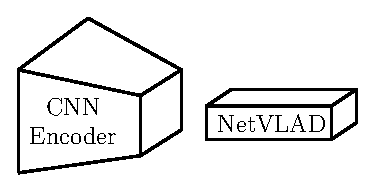
\includegraphics[width=\linewidth]{related_work/enc+vlad}
	
	\caption[]{\label{fig:cnn_aggregation} \textbf{} .}	
	
\end{figure}
\paragraph{Specific architecture.} \label{subsubsec:cnn_aggregation}
\ac{rmac}~\citep{Tolias2016} is an improvement of the precedent \ac{mac} method, consisting of the computation of the \ac{mac} vector over regions of various sizes on the activation map. \citet{Gordo2017} achieve state-of-the-art performances by combining \ac{mac} representation with a custom Region Proposal Network (RPN) that autonomously detects regions of interest on the activation map. They also add a differentiable \ac{pca} layer (implemented with on fully connected layer) for dimension reduction. In~\citep{Radenovic2017}, authors use \ac{gem} pooling, a trade of between mean and max pooling with a trainable parameter controlling the degree of spatial ``focus'' of the network. An entirely trainable aggregation layer, called NetVLAD, have been proposed in~\citep{Arandjelovic2017}. Authors design a differentiable architecture that aim to mimic \ac{vlad} aggregation scheme. In~\citep{Iscen2017}, authors create panorama features by aggregating multiple NetVLAD descriptor in a memory vector. \citet{Kim2017a} use the NetVLAD aggregation layer coupled with an Contextual Reweighing Network (CRN) to downgrade irrelevant features according to their local neighborhood, without the use of any manually annotated data. Along the same lines, \citet{Noh2017} propose the DELF architecture for local features extraction. DELF relies on a self-spatial-attention mechanism to select discriminative local region on the features block. 

\begin{figure}
	\centering

	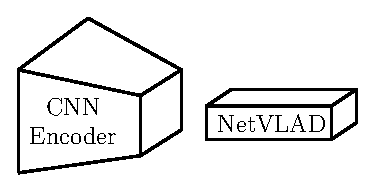
\includegraphics[width=\linewidth]{related_work/enc+vlad}
	
	\caption[]{\label{fig:triplet_ex} \textbf{} .}	

\end{figure}
\paragraph{Training routine}
In recent works~\citep{Arandjelovic2017,Radenovic2016, Gordo2016}, authors tackle the problem of fine tuning a pre-trained network for the specific task of similar images association for localization. The shared idea is to construct images triplet composed of an anchor, a positive example (displaying the same scene as the anchor image with small view point or illumination variation) and a negative example (unrelated to the anchor image). Example of triples are presented in figure~\ref{fig:triplets_ex}. Then, the training signal aims to enforce similarity between computed embedding of the anchor and the positive example and, conversely, to make the anchor and the negative descriptors far for each other in the embedding space. \citet{Arandjelovic2017} introduce a weakly supervised training approach, using the Google Time machine engine to automatically create large database of triplets. Work from~\citep{Gordo2017,Noh2017} make use of a large Landmark dataset for triplets creation. In~\citep{Radenovic2016,Radenovic2017}, \ac{sfm} is used to link multiple images over a large panel of places. The geometric verification provided by \ac{sfm} permit to control the overlaps between anchors and positives examples. In metric learning, hard example mining is an crucial step for creating meaningful embedding space. Hard negative mining is performed in~\citep{Arandjelovic2017,Radenovic2017,Gordo2016} by selecting negative examples that are closer to the anchor in the embedding space. \citet{Iscen2018} introduce a manifold distance to compare dataset examples. With a pre-trained model and without any supervision on the training data, they are able to mine more effective examples compare to standard mining methods.

\subsection{Learning with side information}
As mentioned previously, complementary modalities, like geometry or semantic, may not be always available at test time. This could be due to limitation on the computational resources of an embedded system or to the source of the input (different sensor, old data) during the localization process. For this reason, we make available the geometric information used in this work only during the offline training step and we rely on side information learning to benefit from this auxiliary modality at test time. Recent work from~\cite{Li2017b} casts the side information learning problem as a domain adaptation problem, where source domain includes multiple modalities and the target domain is composed of a single modality. Another successful method has been introduced in~\cite{Hoffman2016}: authors train a deep neural network to hallucinate features from a depth map only presented during the training process to improve objects detection in images. The closest work to ours, presented in~\citep{Xu2017b}, uses recreated thermal images to improve pedestrian detection on standard images only. Our system, inspired by~\citep{Xu2017b}, learns how to produce depth maps from images to enhance the description of these images.

\paragraph{Depth from monocular image for localization.} Modern neural networks architectures can provide reliable estimation of the depth associated to monocular image in a simple and fast manner~\citep{Eigen2014, Godard2017, Mahjourian2018}. This ability of neural networks has been used in~\citep{Tateno2017} to recover the absolute scale in a \ac{slam} mapping system. \citet{Loo2019} use the depth estimation produced by a CNN to improve a visual odometry algorithm by reducing the incertitude related to the projected 3D points. In this work, we use the depth information obtained by a neural network as stable features across season changes. \citet{Taira2019} rely on dense surface normal (derivative of the depth map) and semantic segmentation created by a convolutional encoder/decoder~\citep{Zamir2018} for localization of indoor images with few textures.